\chapter{Pilha}

A pilha é uma estrutura de dados que manipula uma coleção de elementos com duas operações principais:

\begin{itemize}
\item push: que adiciona um elemento na coleção.
\item pop: que remove o elemento que ainda não foi removido adicionado mais recentemente.
\end{itemize}

%Na pilha, a ordem em que os elementos saem da pilha é conhecida pelo acrônimo LIFO (Last in, First out). 

A ideia da estrutura de dados pilha começou a aparecer na literatura da ciência da computação em 1946 com Alan Turing no relatório com o título Propostas para Desenvolvimento na Divisão de Matemática de uma Máquina Automática de Computação\footnote{ \url{https://academic.oup.com/comjnl/article-pdf/20/3/269/2256995/200269.pdf}}.
Ele usou os termos enterrar (bury) and desenterrar (unbury) para o gerenciamento das subrotinas. Em 1957, Klaus Samuelson e Friedrich L. Bauer depositaram uma patente com a idéia da pilha. 



Frequentemente, as pilhas são apresentadas como uma pilha de pratos onde os pratos limpos são colocados no topo da pilha. Note que na pilha de pratos, os primeiros pratos que saem da pilha são os últimos que foram empilhados. Essa política de gerenciamento é conhecida como LIFO (Last in, First out).

As pilhas com tamanho dinâmico podem ser implementadas utilizado as listas sequencias com tamanho dinâmico ou listas encadeadas. 

Na linguagem C++, a classe stack suporta as seguintes operações:

\begin{itemize}
\item empty
\item pop
\item push
\item size
\item top
\end{itemize}


Em alguns casos, podemos implementar a classe stack como uma classe derivada diretamente da classe vector.

\begin{minted}{C++}
template <typename T> 
class stack : public std::vector <T>
{
  public:
  using base_type = std::vector <T> ;
  void  push ( const T& x ) { base_type::push_back( x ); }
  const T& top  ()             { return base_type::back(); }
  void  pop  ()             { base_type::pop_back(); }
  bool  empty()             { return base_type::empty(); }
};
\end{minted}

Podemos implementar a classe stack utilizando um vector internamente.

\begin{minted}{C++}
template <typename T> 
class stack 
{
  using base_type = std::vector <T> ;
  private:
    base_type data;
  public:
  void  push ( const T& x ) { data.push_back( x ); }
  const T& top  ()             { return data.back(); }
  void  pop  ()             {  data.pop_back(); }
  bool  empty()             { return data.empty(); }
};
\end{minted}

\section{Recursão}

As linguagens de programação que suportam recursão utilizam uma pilha de chamada (\textit{call stack}). Para cada chamada de um subprograma, um registro de ativação é criado na pilha de chamadas. No registro de ativação armazenamos algumas informações sobre o subprograma como:

\begin{itemize}
\item parâmetros
\item endereço de retorno
\item valor das variáveis locais 
\end{itemize}

Quando o subprograma não está mais ativo, essas informações deixam de ser armazenadas. 

Considere o seguinte programa recursivo:

\begin{minted}{C++}
int fact(int n){
    if(n==1)
        return 1;
    else
        return n*fact(n-1);
}
\end{minted}

A Figura abaixo mostra de maneira simplificada como a pilha de ativação é alterada para o cálculo de fact(3). 

\begin{figure}[htbp]
\centering
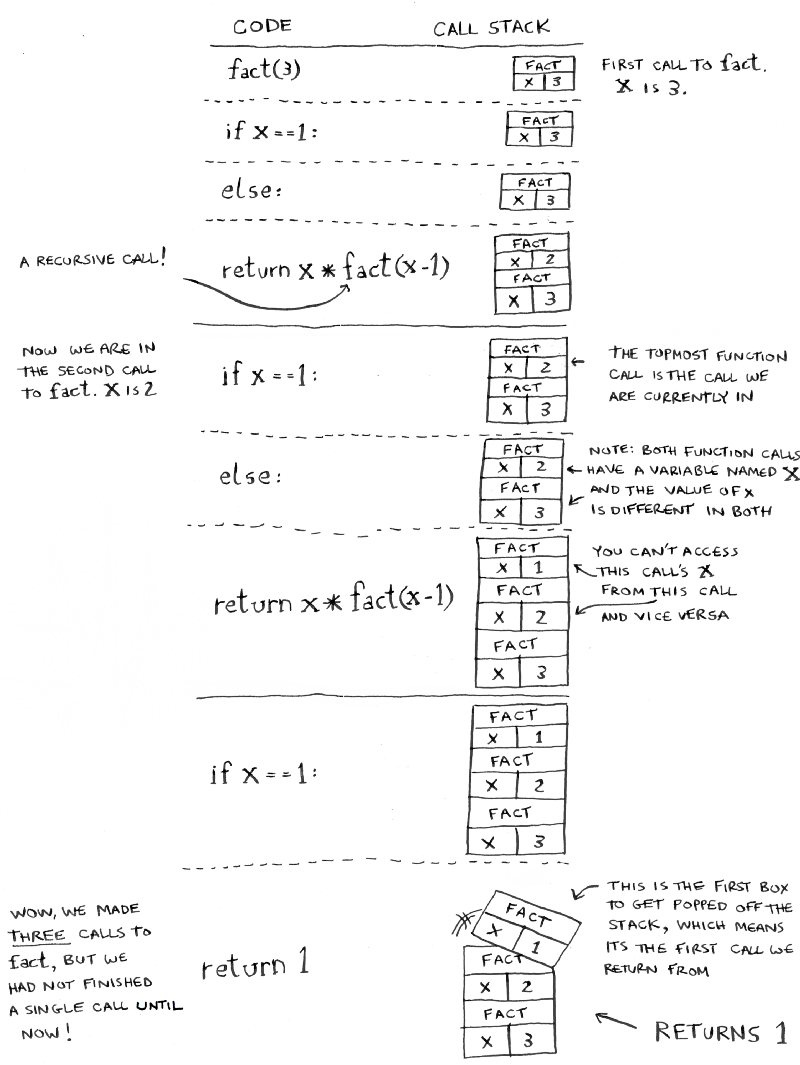
\includegraphics[scale=0.4]{images/callstack.png}
\caption{Image credit: Adit Bhargava} 
\end{figure}

\newpage 


O site Pythontutor permite também visualizar a pilha de chamadas de maneira simplificada.

\begin{figure}[htbp]
\centering
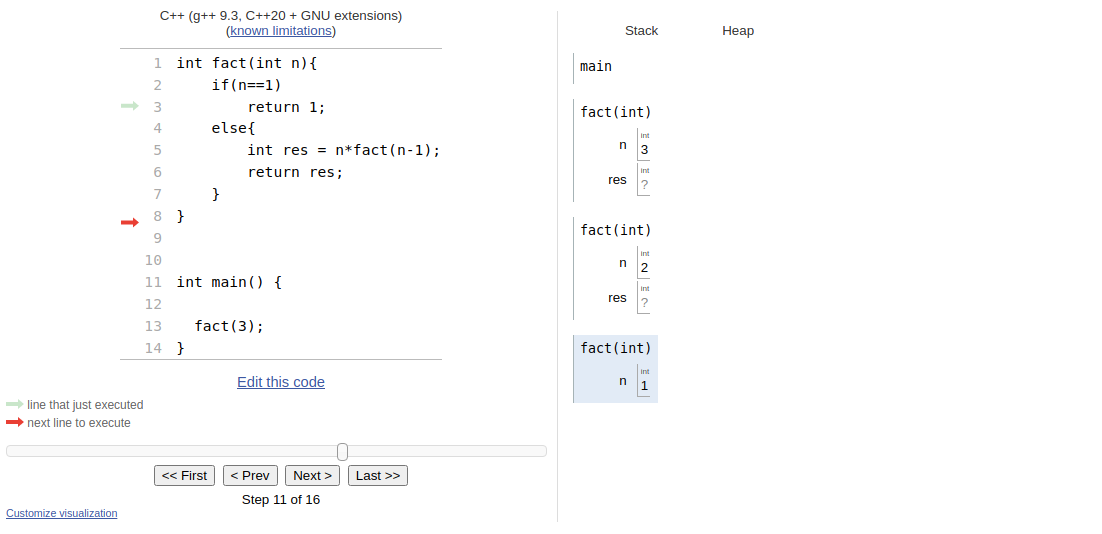
\includegraphics[scale=0.5]{images/pythontutor.png}
\caption{site pythontutor.com}
\end{figure}


Todo programa recursivo pode ser simulado utilizando uma pilha. Por exemplo, o programa fatorial pode ser simulado utilizando pilha da seguinte maneira:

\begin{minted}{C++}
int fact(int n){
    stack <int> s;
    while(n>1){
        s.push(n);
        n--;
    }
    int ret = 1; // caso base
    while( !s.empty() ){
        int u = s.top();
        ret = u*ret;
        s.pop();
    }
    return ret;
}
\end{minted}

No código seguinte, vamos simular o fatorial utilizando uma pilha de funções. Vamos empilhas as funções $n*,(n-1)*, \ldots ,2*$. Em seguida, vamos plugando o resultado obtido pela função desempilhada.

\begin{minted}{C++}

auto f(int a){
    return [=](int b){ return a*b; };
}
stack <  function<int(int)> > s;
void push(int n){
    while(n > 1){
        s.push(f(n)); // push n*
        n--;
    }
}
int calc_fact(int n){
    push(n);
    
    /*
    stacking
    2*
    .
    .
    .
    n-2*
    n-1*
    n*
    */

    int ret = 1;
    while( !s.empty() ){
        auto g = s.top();
        ret = g(ret); 
        s.pop();
    }
    return ret;
}
\end{minted}

\section{Fibonacci}

Considere o programa recursivo para o número de fibonacci:

\begin{minted}{C++}
int fibonacci(int n){
    if(n==1 || n == 2) return n;
    else return fibonacci(n-1) + fibonacci(n-2);
}
\end{minted}

Dessa vez, vamos simular o programa recursivo com duas pilhas. Uma pilha de operações que devem ser realizadas e uma pilha de valores de retorno.

\begin{minted}{C++}
enum class optype { sum, calc };
class Operation{
    public:
    optype op;
    int n;
    Operation(optype t, int v = 0): op(t), n(v) {} 
};

int calc_fibonacci(int n){
    stack <Operation> s;
    stack <int> ret;
    s.push( Operation(optype::calc, n) );
    while( !s.empty() ){
        auto u = s.top();
        s.pop();
        if( u.op == optype:: calc )
        {
            if( u.n == 1 || u.n == 2 ){
                ret.push(u.n);
            }else{
                s.push( Operation( optype::sum )      );
                cout << "pushing sum" << endl;
                s.push( Operation( optype::calc, u.n-1) );
                cout << "pushing calc " << u.n-1 << endl;
                s.push( Operation( optype::calc, u.n-2) );
                cout << "pushing calc " << u.n-2 << endl;   
            }
        } 
        else if( u.op == optype:: sum )
        {         
            int a,b;
            a = ret.top();
            ret.pop();
            cout << "popping " << a << endl;
            b = ret.top();
            cout << "popping " << b << endl;
            ret.pop();
            ret.push(a+b);
            cout << "pushing " << a+b << endl;
            
        }
        
    }
    return ret.top();
}
\end{minted}

No cálculo do fibonacci(6), temos o programa escreve as seguintes mensagens:

\begin{minted}{C++}
pushing sum
pushing calc 5
pushing calc 4
pushing sum
pushing calc 3
pushing calc 2
pushing sum
pushing calc 2
pushing calc 1
popping 2
popping 1
pushing 3
popping 3
popping 2
pushing 5
pushing sum
pushing calc 4
pushing calc 3
pushing sum
pushing calc 2
pushing calc 1
popping 2
popping 1
pushing 3
pushing sum
pushing calc 3
pushing calc 2
pushing sum
pushing calc 2
pushing calc 1
popping 2
popping 1
pushing 3
popping 3
popping 2
pushing 5
popping 5
popping 3
pushing 8
popping 8
popping 5
pushing 13


\end{minted}




\section{Algoritmo Shunting Yard}

O algoritmo Shunting Yard foi proposto por Edsger Dijkstra em 1961 para converter uma expressão infixa em uma expressão na notação polonesa reversa usando pilha. 

A notação polonesa foi proposta pelo lógico polonês Jan Łukasiewicz em 1924. Nessa notação, os operadores aparecem antes dos seus operandos.

Já a notação polonesa reversa foi proposta em 1954 por Arthur Burks, Don Warren e Jesse Wright e de maneira independente em 1961 por Friedrich L. Bauer e Edsger W. Dijkstra para auxiliar no processo de avaliação de expressões nas linguagens de programação.


Na notação polonesa reversa, primeiramente escrevemos os operandos em seguida os operadores. A notação polonesa reversa possui duas vantagens principais:

\begin{enumerate}
\item A expressão não precisa utilizar os parênteses uma vez que cada operador tem um número fixo de operandos.
\item As regras de associatividade e precedência não precisam ser definidas.
\end{enumerate}

Por exemplo, a expressão A + B * C fica A B C * +.

O processo de conversão da expressão infixa para a expressão na notação polonesa reversa pode ser realizada pela seguintes regras.

\begin{enumerate}
\item Se o símbolos da entrada forem um operando, imprima-o.

\item Se o símbolo da entrada for um parêntese esquerdo, empilhe-o na pilha.

\item Se o símbolo da entrada for um parêntese direito: descarte o parêntese direito, desempilhe e imprima os símbolos da pilha até ver um parêntese esquerdo. Desempilhe o parêntese esquerdo e descarte-o.

\item Se o símbolo da entrada for um operador e a pilha estiver vazia ou contiver um parêntese esquerdo no topo, empilhe o operador da entrada para a pilha.

\item Se o símbolo da entrada for um operador e tiver precedência mais alta do que o operador no topo da pilha, ou tiver a mesma precedência do operador no topo da pilha e for associativo à direita - empilhe-o na pilha.

\item Se o símbolo da entrada for um operador e tiver precedência inferior ao operador no topo da pilha, ou tiver a mesma precedência do operador no topo da pilha e for associativo à esquerda - continue a desempilhar da pilha até que seja verdade. Em seguida, empilhe o operador de entrada.

\item No final da expressão, desempilhe e imprima todos os operadores na pilha. (Nenhum parêntese deve permanecer.)

\end{enumerate}

Nos exemplos seguintes utilizaremos, o símbolo \$ para representar o final da expressão.

\begin{exemplo}
Considere o processo de conversão da seguinte expressão A + B * C\$.

\begin{tabular}{llll}
  &Símbolo da Entrada    & Pilha  & Notação Polonesa Reversa \\
1 & A     &    & A \\
2 & +     & +  & A \\
3 & B     & +  & A B\\
4 & *     & + *  & A B\\
5 & C     & + *  & A B C\\
6 & \$     &    & A B C * +\\

\end{tabular}


\end{exemplo}


\begin{exemplo}
Considere o processo de conversão da seguinte expressão A * (B + C * D) + E\$.

\begin{tabular}{llll}
  &Símbolo da Entrada    & Pilha  & Notação Polonesa Reversa \\
1 & A     &    & A \\
2 & *     & *  & A \\
3 & (     & * ( & A \\
4 & B     & * (  & A B\\
5 & +     & * ( +  & A B\\
6 & C     & * ( +   & A B C\\
7 & *     & * ( + *   & A B C\\
8 & D     & * ( + *   & A B C D\\
9 & )     & *    & A B C D * + *\\
10 & +    & +    & A B C D * + * \\
11 & E    & +    & A B C D * + * E\\ 
12 & \$   &     & A B C D * + * E +\\ 

\end{tabular}


\end{exemplo}


\textbf{Exercício:}

\begin{enumerate}
    \item Dado uma expressão na notação polonesa reversa com os operadores +,-,*,/ calcule o valor da expressão utilizando uma pilha.
\end{enumerate}




\section{Stack-Insertion Sort}

O algoritmo Stack-Insertion Sort pode ser implementado utilizando duas pilhas chamadas esquerda e direita. A pilha esquerda é usada para empilhar os itens em ordem crescente, enquanto a pilha da direita é usada para empilhar os elementos em ordem decrescente. O topo de cada pilha no passo i representa o ponto de inserção do elemento i. A pilha da esquerda começa empilhando o menor valor ($-\infty$) e pilha direita começa empilhando o maior valor ($+ \infty$).  


O algoritmo Stack-Insert Sort pode ser implementado da seguinte maneira:

\begin{algorithm}
\caption{Stack-Insert Sort}
\begin{algorithmic}

\State $i \gets 1$
\State esquerda.push($-\infty$)
\State direita.push($+\infty$)

\While{ $i \leq n$}
    
    \If{$a_i$ $<$ esquerda.top()}
    \While{ $a_i < $ esquerda.top()}
    \State direita.push(esquerda.top())
    \State esquerda.pop()
    \EndWhile
    \State esquerda.push($a_i$)
    \Else
        \If{$a_i$ $<$ direita.top()}
        \State direita.push($a_i$)
        \Else
            \While{ $a_i > $ direita.top()}
            \State esquerda.push(direita.top())
            \State direita.pop()
            \EndWhile
            \State direita.push($a_i$)
        \EndIf
    \EndIf
    
    
    \State $i \gets i + 1$
    
\EndWhile

\While { direita.top() $\neq +\infty$ }
\State esquerda.push(direita.top())
\State direita.pop()
\EndWhile 
\end{algorithmic}
\end{algorithm}

\begin{exemplo}
Execução do algoritmo Stack-Insert Sort para o vetor a = [20,67,07,31,53,11,6,55]

\begin{tabular}{lll}
\hline
         & a        &   20 67 07 31 53 11 6 55        \\
passo 0  &   esquerda & $-\infty$                                \\
         & direita  & $+\infty$\\
\hline
         & a        &   67 07 31 53 11 6 55        \\
passo 1  &   esquerda & $-\infty$                                \\
         & direita  & $+\infty$ 20\\
\hline
         & a        &   07 31 53 11 6 55        \\
passo 2  &   esquerda & $-\infty$ 20                               \\
         & direita  & $+\infty$ 67\\
\hline
         & a        &   31 53 11 6 55        \\
passo 3  &   esquerda & $-\infty$ 07                                \\
         & direita  & $+\infty$ 67 20\\
\hline
         & a        &   53 11 6 55        \\
passo 4  &   esquerda & $-\infty$ 07 20                               \\
         & direita  & $+\infty$ 67 31\\
\hline
         & a        &   11 6 55        \\
passo 5  &   esquerda & $-\infty$ 07 20 31                               \\
         & direita  & $+\infty$ 67 53\\
\hline
         & a        &   6 55        \\
passo 6  &   esquerda & $-\infty$ 07 11                                \\
         & direita  & $+\infty$ 67 53 31 20 \\
\hline
         & a        &   55        \\
passo 7  &   esquerda & $-\infty$ 06                                \\
         & direita  & $+\infty$ 67 53 31 20 11 07\\
\hline
         & a        &   -        \\
passo 8  &   esquerda & $-\infty$ 06 07 11 20 31 53                                 \\
         & direita  & $+\infty$ 67 55\\
\hline
         & a        &   -        \\
passo 9  &   esquerda & $-\infty$ 06 07 11 20 31 53 55 67                                 \\
         & direita  & $+\infty$ \\
\hline

\end{tabular}
\end{exemplo}
